\documentclass[a4paper]{article}

\usepackage{graphicx}
\usepackage[english]{babel}
\usepackage[utf8]{inputenc}
\usepackage{amsmath}
\usepackage[colorinlistoftodos]{todonotes}

\title{Software Architecture Design}

\author{Group 6}

\date{\today}

\begin{document}
\maketitle
\begin{center}
D Doman [11002566]\\
P Hammond [11025477]\\
BW M$\ddot{u}$ller [11037157]\\
JF Oberholzer [12039803]\\
AD Pretorius [12022404]\\
ER Rosslee [12223426]\\
R Schnetler [12220702]\\
\textbf{Git Repository: } \texttt{https://github.com/BWMuller/COS301-MiniProject-G6-P2}

\end{center}
\pagebreak

\section{Software Architecture Design}

This section discusses the software architecture requirements. It will specify how the software infrastructure that is to be developed will address the functional requirements. All of this is done within the architecture constraints given by the client. What follows is firstly a summary of the functional requirements, then a summary of the constraints given by the client, then a list of the chosen technologies, frameworks, protocols and libraries and a justification of why that choice was made and how it addresses the problem. 

\section{Functional Requirements}

\subsection{Access}

The system will be accessible by humans from a browser through a rich web interface, this interface must be accessible through all recent versions of mayor browsers. There must also be an Adriod application to be accessed through mobile Android devices with all recent versions of Android.
	
\subsection{Integration}

The system must access a UP CS server and database to retrieve students' personal information and access course information. The server is LDAP and the database is MySQL. When the marks are exported that should be done in a CSV file. All communication must be done using secure HTTPS.

\subsection{Security}

Users must authenticate to the LDAP server before using any of the services. The service should also ensure that users only access the parts that they have access to. 
	
\subsection{Auditability}

The system should keep track of any changes made to any entity in the database. It should record who makes that change, when do they make it and from what to what it was changed. The audit log cannot be modified.

\subsection{Testability}

All the services offered by the system should be testable. It should test if the service is provided under the right conditions and that post-conditions hold true after service has been provided. 

\subsection{Usability}

The software should be easy to understand and use without prior training. It should be in English but it should be open to be translated to other languages.

\subsection{Scalability}

The system should be open to be scaled and expanded to hadle all the assesments for all the modules of the Department of Computer Science. The system should be able to hanle 100 users at the same time.
	
\subsection{Performance}

All non-reporting operations should report within less than 1 second. Report queries should be processed in no more than 10 seconds.

\section{Architecture Constraints}
	
The system should be developed using the Django web framework. Persistence to a relational database must be done using the Object-Relational Mapper bundled with Django. The Django unittest module should be used for testing. The system should be deployed on a Django application server running within the cs.up.ac.za Apache web server. The mobile client should be running on an Android application. The system will use the MySQL database. Web services must be either SOAP-based or Restful web services.

\section{Architecture Design}

\subsection{Access}

There should be a web application and a mobile application. For the web application we are going to use the Djanga Web Framework. This is the framework that the users wants, but also has many advantages. Django works with Python, one of the simplest programming languages out there. The structure is also very good and resolves around building the website in phases. Django also adheres strongly to the DRY (Don't repeat yourself) principle. For the mobile app we will use Android, since it is the most popular mobile OS out there.

\subsection{Integration}

The CS server already uses MySQL and so we will keep consistency and also use this. MySQL is also cost effective since it is open source. MySQL can work cross platform and has good security. We will also use the Object-Relational Mapper bundled with Django since we use Django.

\subsection{Security}

The security of MySQL is very, very good. The server has its own security, then the database has more security.

\subsection{Auditability}

Using the Django framework we will create an auditability program that will keep track of all the changes and store it on the server.

\subsection{Testability}

The Django framework includes a unittest module we can use to thouroughly test this system.

\subsection{Usability}

We will apply proper design principles like affordances to make the system clear and easy to use.

\subsection{Scalability}

Both Django and MySQL are scalable to the level we desire.
        
\subsection{Performance}

Both Django and MySQL can perform to the level we desire.

\section{Application Design}
\subsection{The Back-End System}
\subsection*{Specifications of Lower Levels of Granularity}
\subsection*{Mobile}
\begin{itemize}
\item \textbf{Interface}: Implements an interface to the system from the API (andoid.view). 
\item \textbf{Communication}: This is accomplished by using client server communication (secure script protocols).  The communication must be done by implementing the Android API client side.
\item \textbf{API}:  Interactions to the interface must be done using the android.gesture class.
\item All interactions must be validated and audited server-side.
\end{itemize}

\subsection*{User Login}
\begin{itemize}
\item \textbf{Back End}: Receives user login information and confirms its validity using a compare functionality outside the Database interaction.
\end{itemize}

\subsection*{Leaf Assessment}
\begin{itemize}
\item \textbf{Back End}: Get information on a leaf with condition to either create, delete or update. It the performs the operation and returns the success of the operation
\end{itemize}

\subsection*{Aggregate Assessment}
\begin{itemize}
\item \textbf{Back End}: Get details of aggregation and applies them to relevant leaf and returns the result of the aggregation.
\end{itemize}

\subsection*{Assessment Report}
\begin{itemize}
\item \textbf{Back End}: Receives the details specifying the range of assessments to include and collect all the relevant data and transmit it back.
\end{itemize}

\subsection*{Student Report}
\begin{itemize}
\item \textbf{Back End}: Receives the student details and collects the data required and returns it.
\end{itemize}

\subsection*{Audit Report}
\begin{itemize}
\item \textbf{Back End}:  Gathers the data for the required Audit and includes all default and relevant log information and returns the collection.
\end{itemize}

\subsection*{API Specifications}

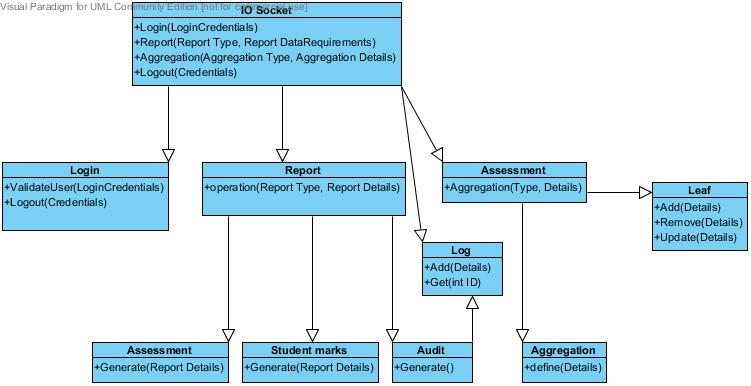
\includegraphics[width=400px]{Images/APIBackEnd1.jpg}
\begin{center}
Figure 1: Back-End API Specification
\end{center}

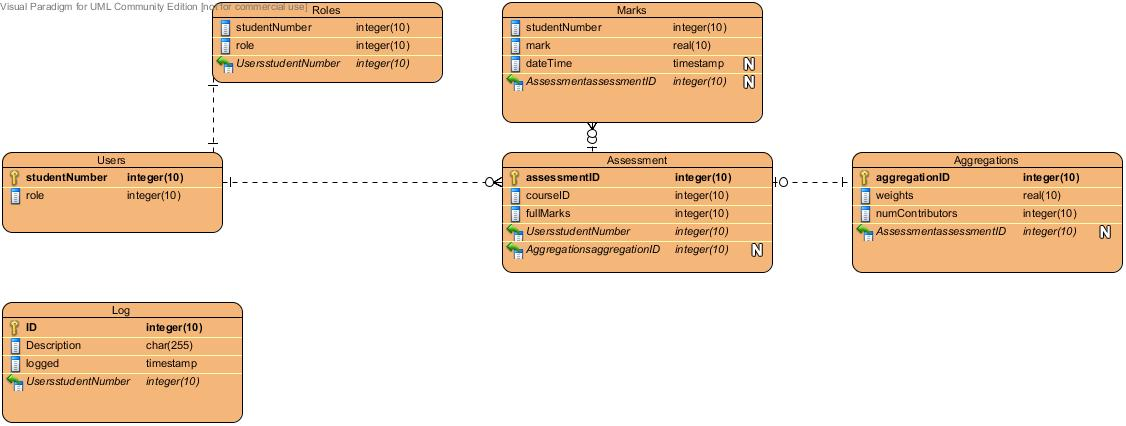
\includegraphics[width=400px]{Images/APIBackEnd2.jpg}
\begin{center}
Figure 2: Back-End Entity Relationships
\end{center}

\subsection{Web Application}
The web application of the Squirrel Marking System provides a browser-based user interface in the application.

\subsection*{Lower Levels of Granularity}
The lower levels of granularity consists of 3 main users:

\textbf{Student}: This user is first required to log in before he/she can use the system. The only functions  permitted to the student to perform on this system is to view his registered modules' 	marks and render his marks onto the web screen, CSV or PDF file.

\textbf{Marker}: This user is also required to log in before he/she can use the system. A marker can be a 	lecturer or student. A marker can only mark leaf or aggregate assessments of certain students. He can submit,add,modify and delete students' marks.

\textbf{Lecturer}: This user is also required to log in before he/she can use the system. The lecturer is by default also a marker.The lecturer can define and control assessments,that is he/she can   		create,modify and delete assessments as well as create, modify, lock and unlock assessment sessions. He/she can also generate reports for a specified assessment, specified student or audit log , having it rendered on the web user interface, CSV or PDF document and publish students' marks.

\subsection*{User Work Flow Diagrams}
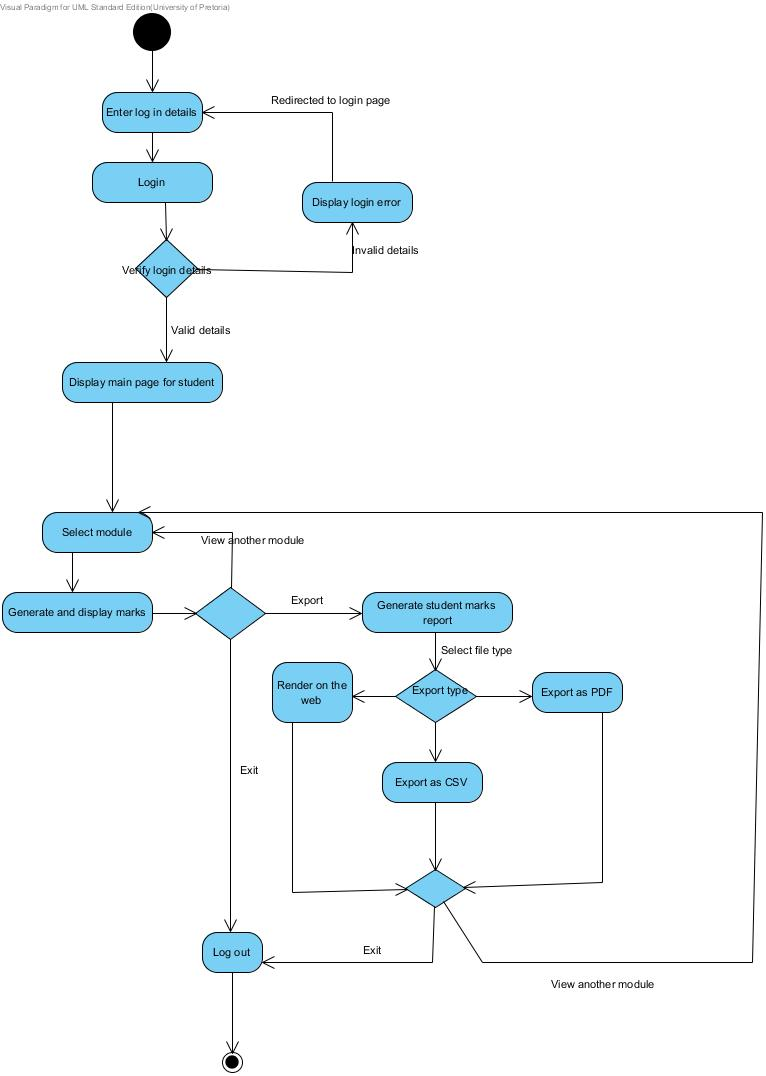
\includegraphics[width=380px]{Images/WEBUWStudentActivity.jpg}
\begin{center}
Figure 3: Activity Diagram for the Student.
\end{center}
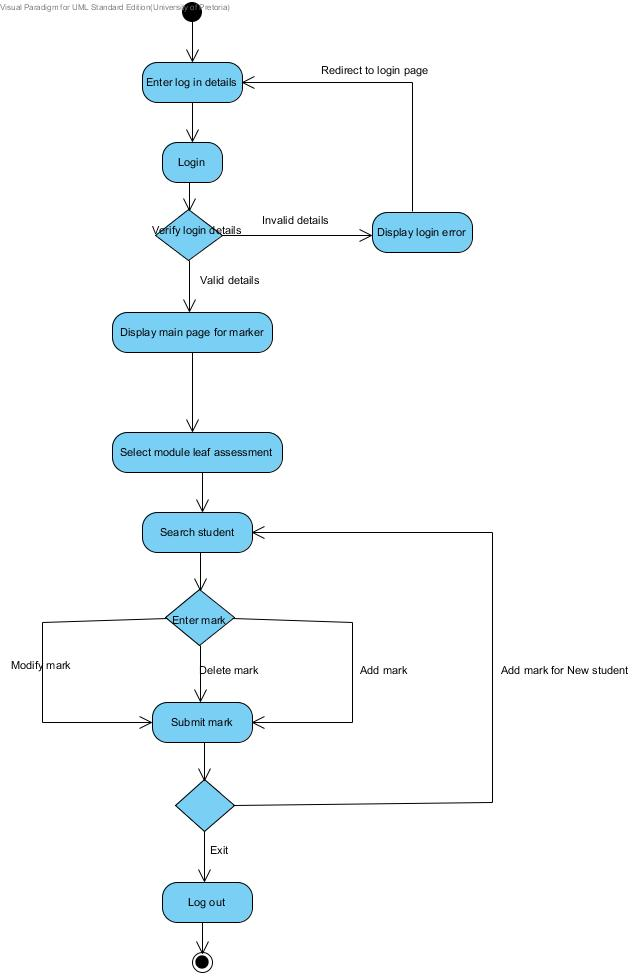
\includegraphics[width=380px]{Images/WEBUWMarkerActivity.jpg}
\begin{center}
Figure 4: Activity Diagram for the Marker.
\end{center}
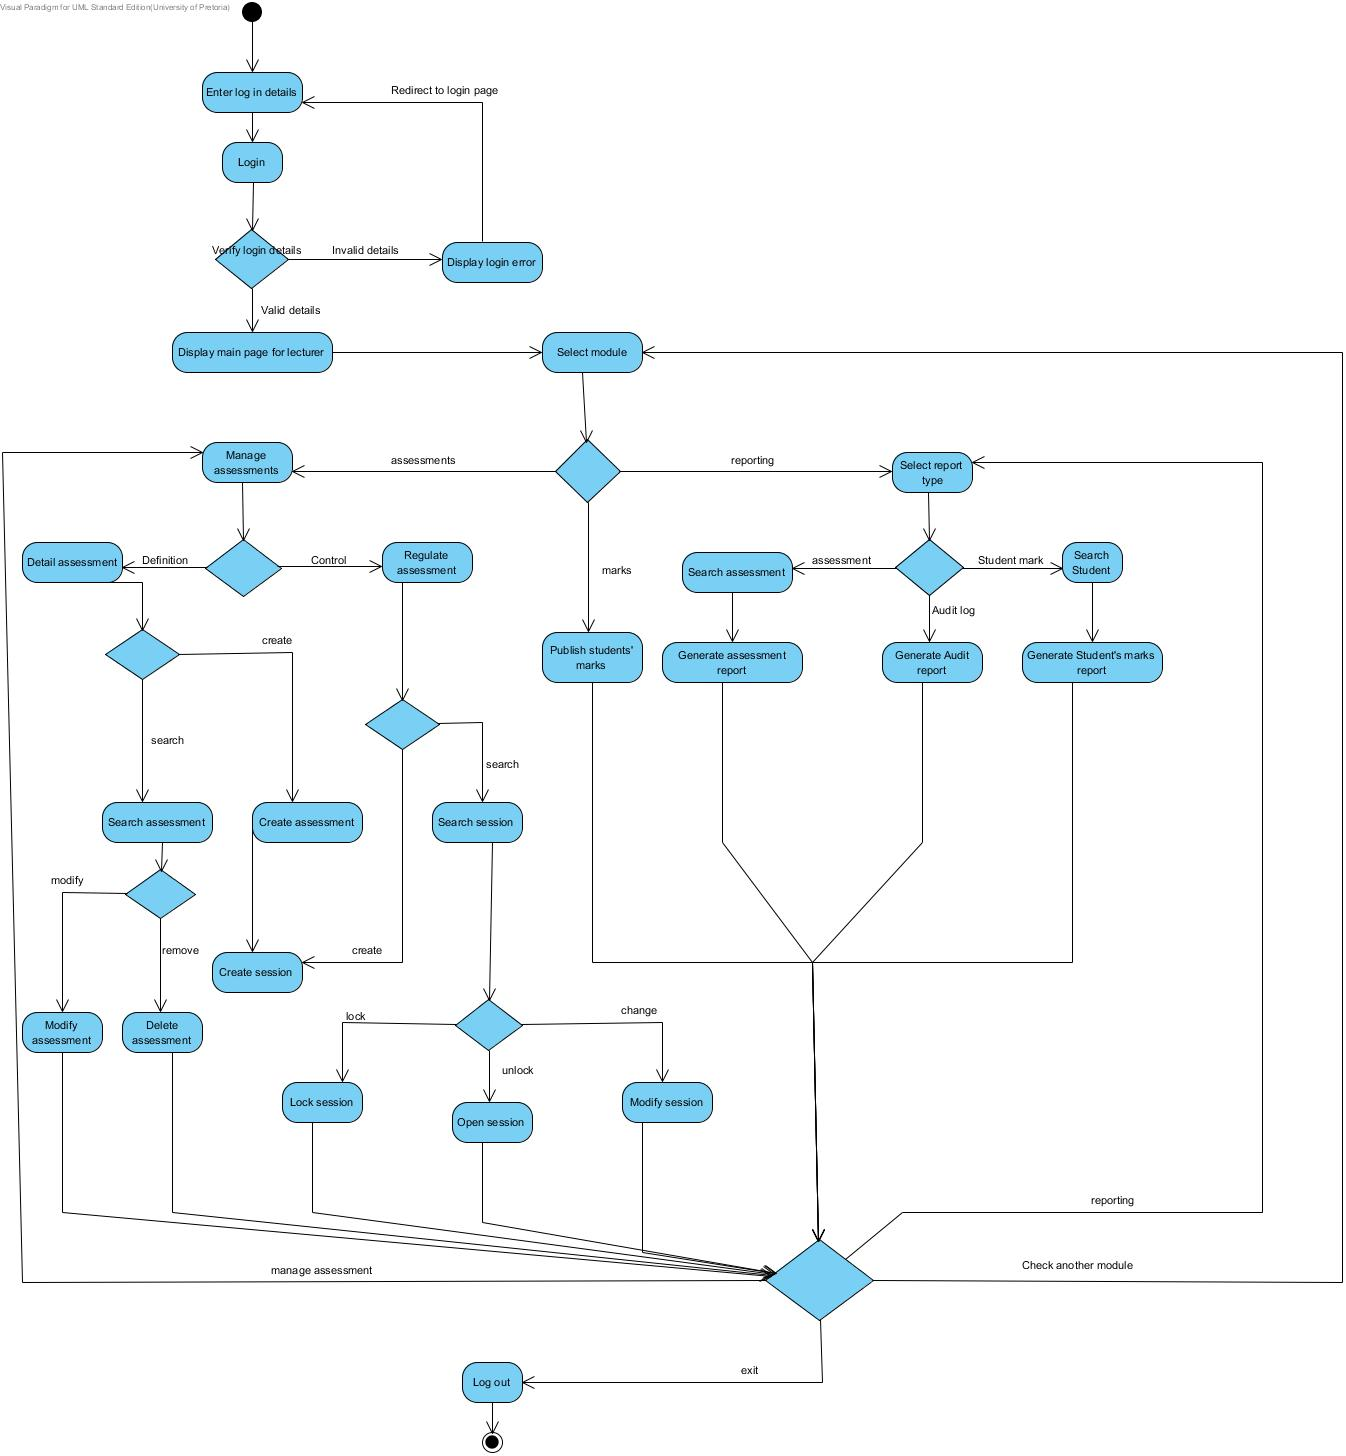
\includegraphics[width=380px]{Images/WEBUWLecturerActivity.jpg}
\begin{center}
Figure 5: Activity Diagram for the Lecturer.
\end{center}

\subsection*{User Interface Diagrams}
\includegraphics[width=380px]{Images/WEBUILogin.jpg}
\begin{center}
Figure 6: The Login Screen where a lecturer or student logs in using his/her CS details
\end{center}
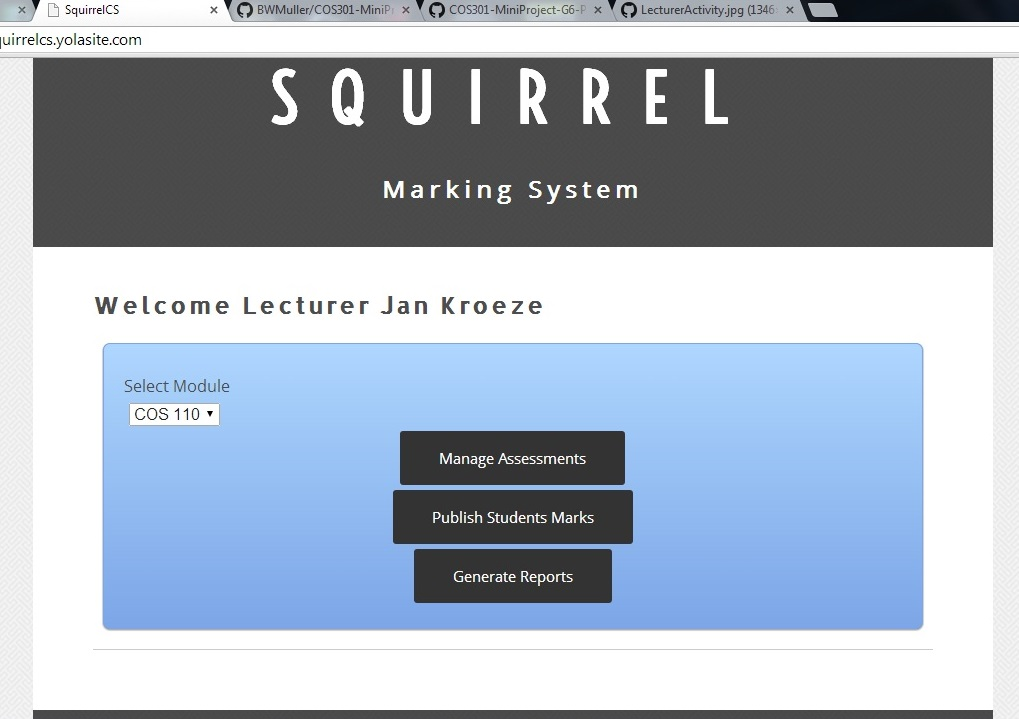
\includegraphics[width=380px]{Images/WEBUILecturer_SelectModule.jpg}
\begin{center}
Figure 7: If a lecturer logs in, he/she chooses a module from a list of modules that they are teaching.
\end{center}
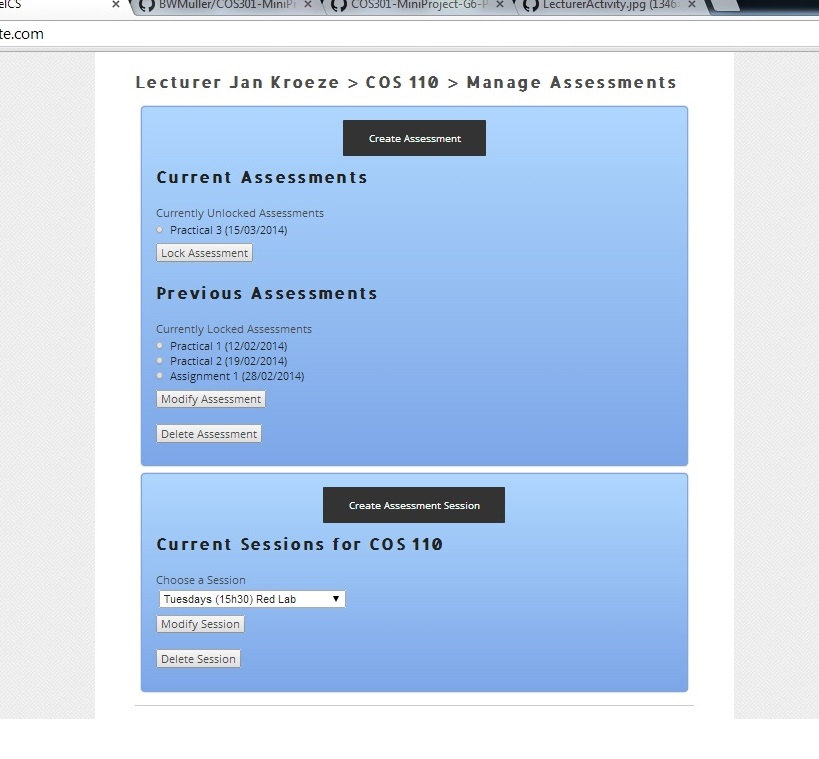
\includegraphics[width=380px]{Images/WEBUILecturer_ManageAssessment.jpg}
\begin{center}
Figure 8: The lecturer then can choose to manage an assessment for that module.
\end{center}
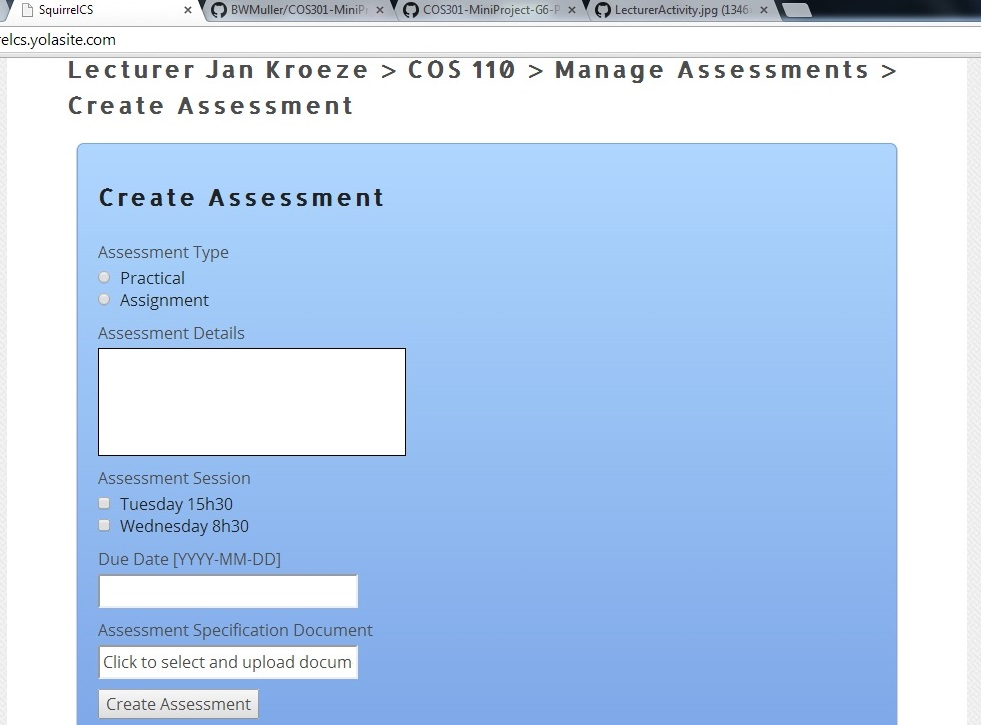
\includegraphics[width=380px]{Images/WEBUILecturer_CreateAssessment.jpg}
\begin{center}
Figure 8: A lecturer can create or modify an assessment.
\end{center}
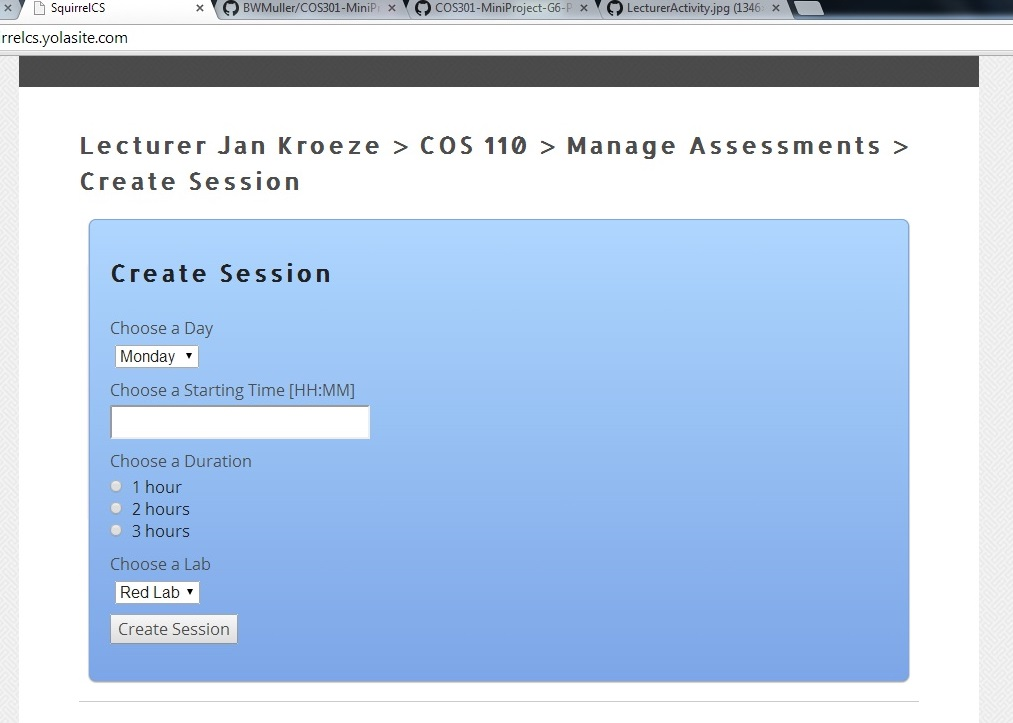
\includegraphics[width=380px]{Images/WEBUILecturer_CreateSession.jpg}
\begin{center}
Figure 9: A lecturer may also create or modify a marking session.
\end{center}
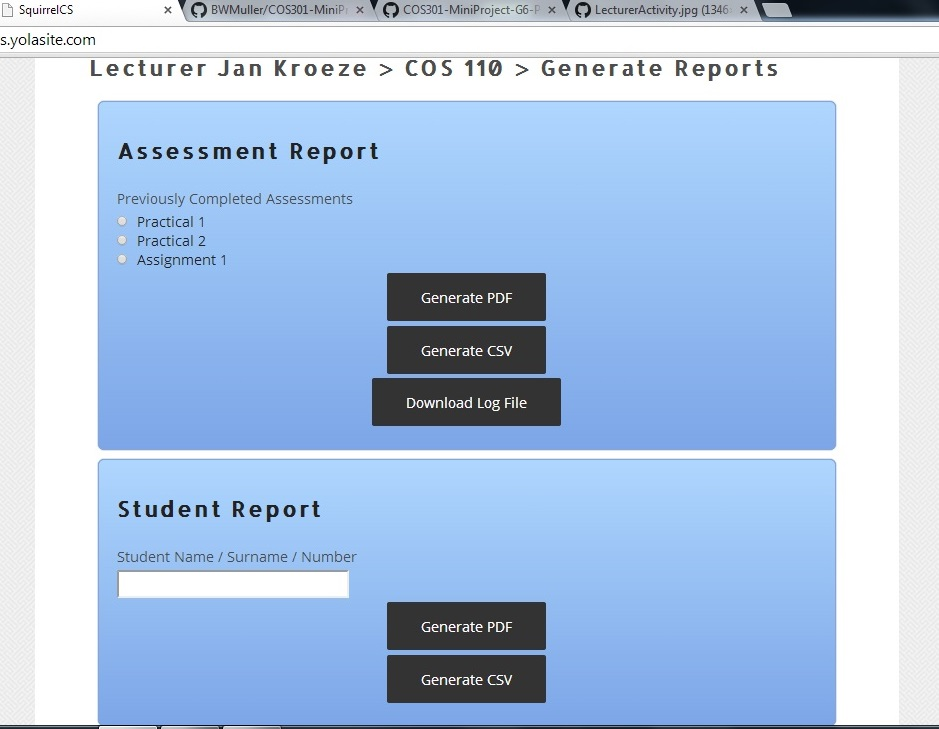
\includegraphics[width=380px]{Images/WEBUILecturer_GenerateReprots.jpg}
\begin{center}
Figure 10: The lecturer can also download reports on assessments or individual student marks as PDF or CSV files.
\end{center}
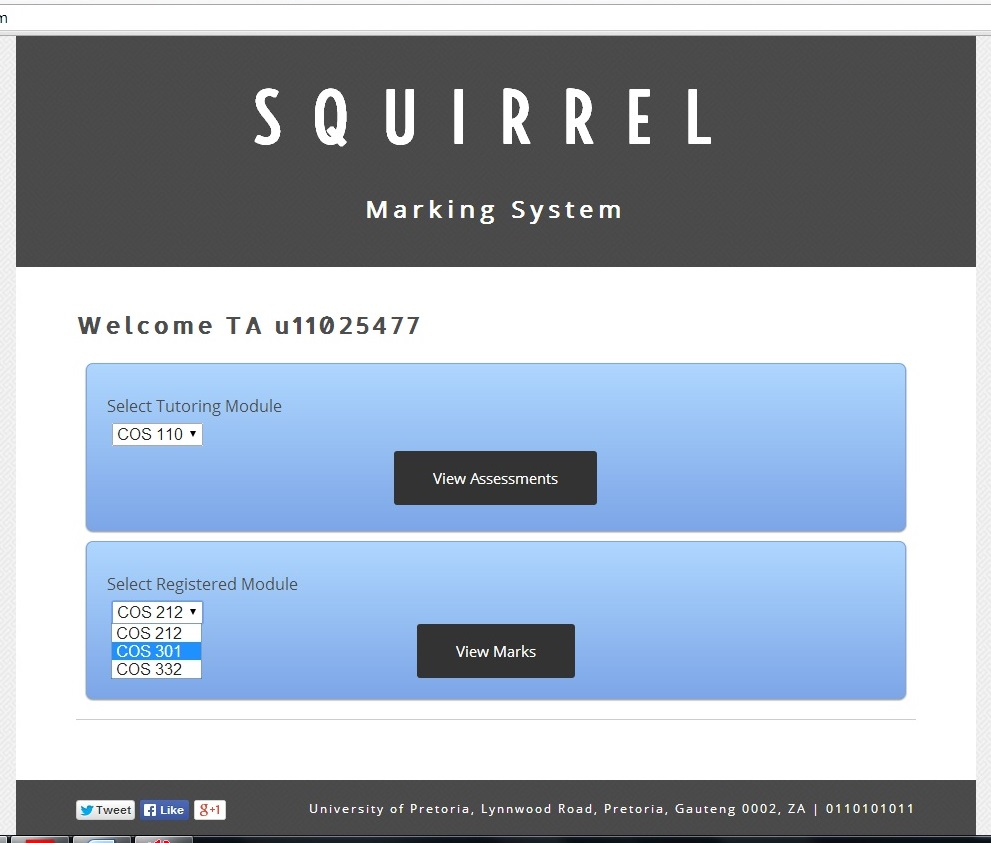
\includegraphics[width=380px]{Images/WEBUITA_SelectModule.jpg}
\begin{center}
Figure 11: When a TA logs in , they either choose a module for which they are currently registered, or a module they are a TA for.
\end{center}
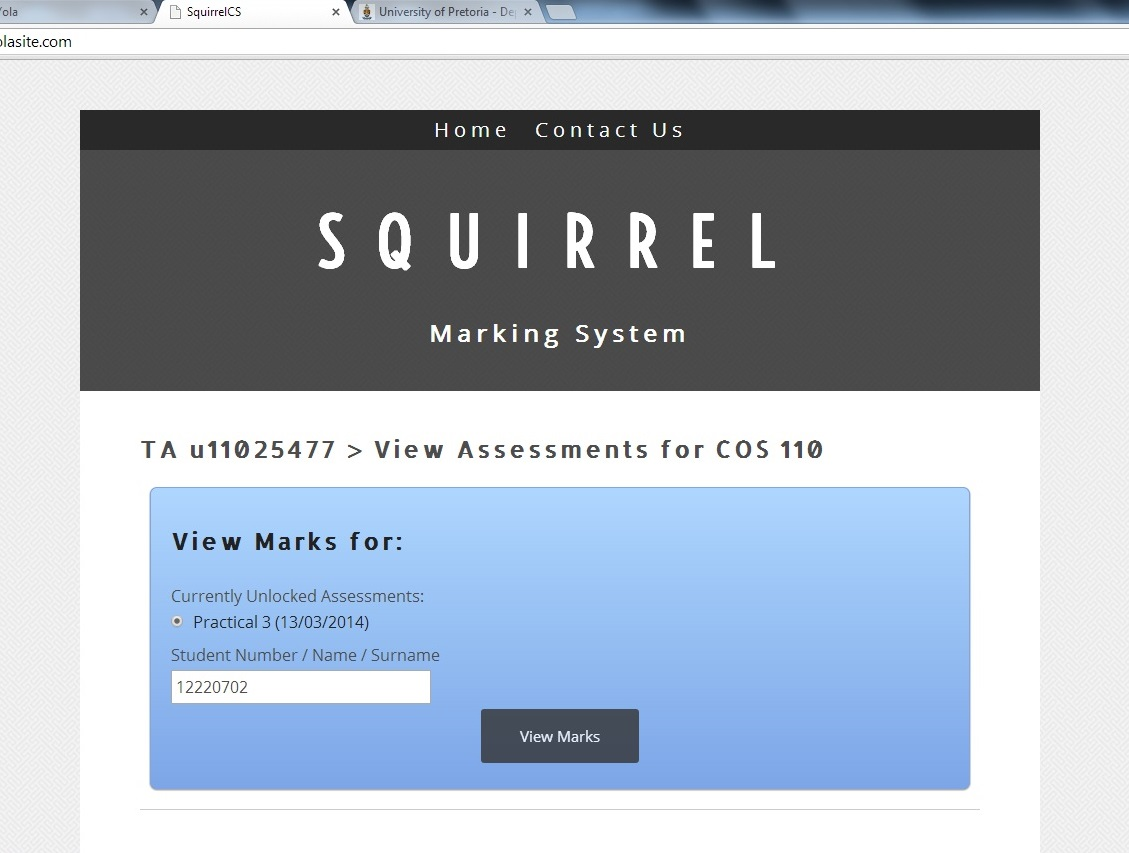
\includegraphics[width=380px]{Images/WEBUITA_ViewAssessments.jpg}
\begin{center}
Figure 12: They can then select the unlocked assessment they are interested in.
\end{center}
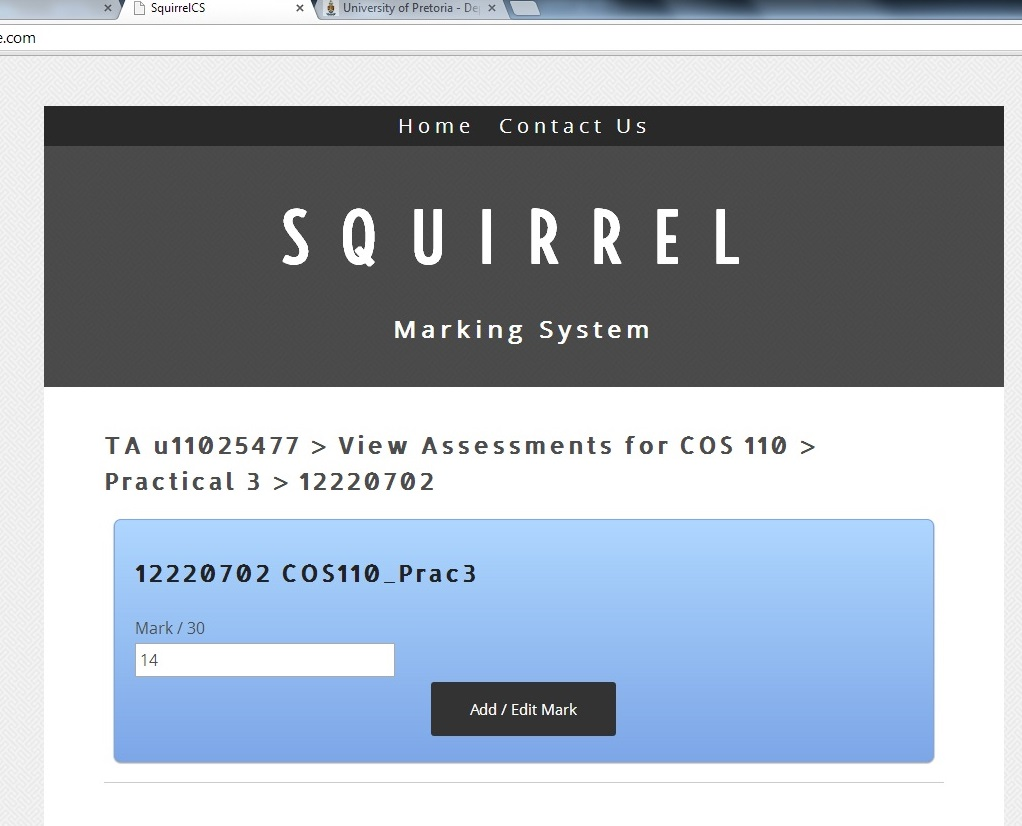
\includegraphics[width=380px]{Images/WEBUITA_ViewAddEditMarks.jpg}
\begin{center}
Figure 13: And then select a student and edit his/her marks.
\end{center}
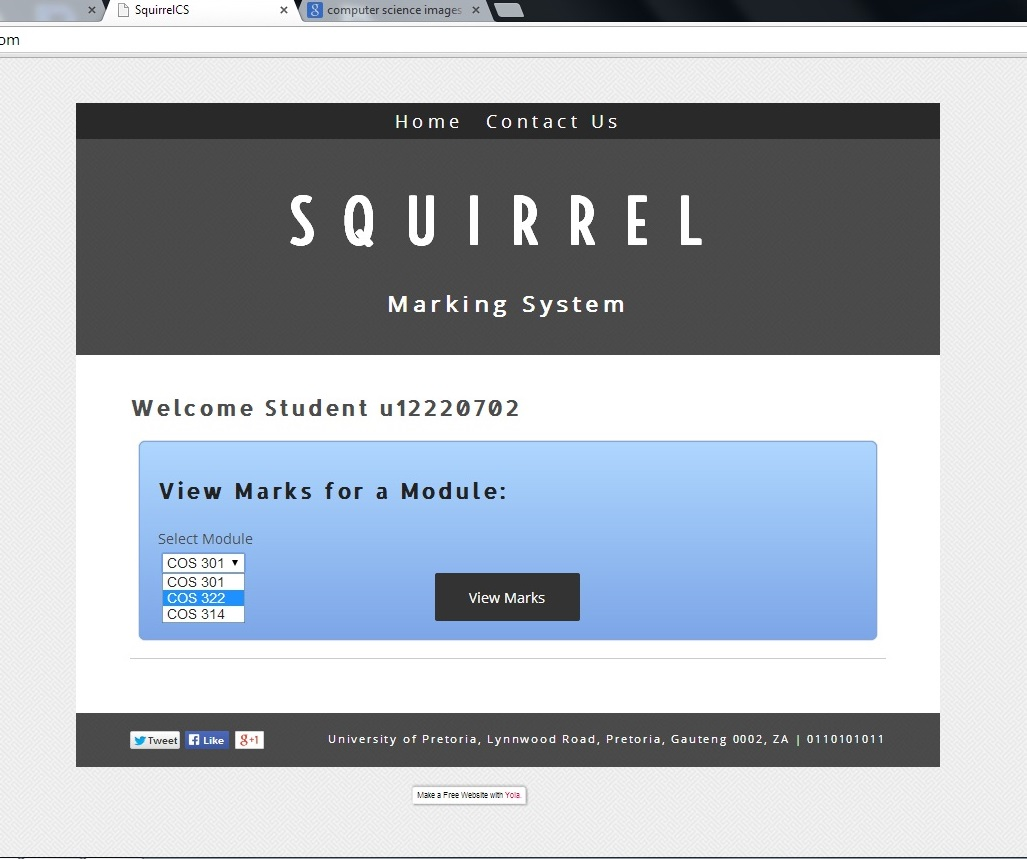
\includegraphics[width=380px]{Images/WEBUIStudent_SelectModule.jpg}
\begin{center}
Figure 14: When a student logs in , they can only select a module they are registered for.
\end{center}
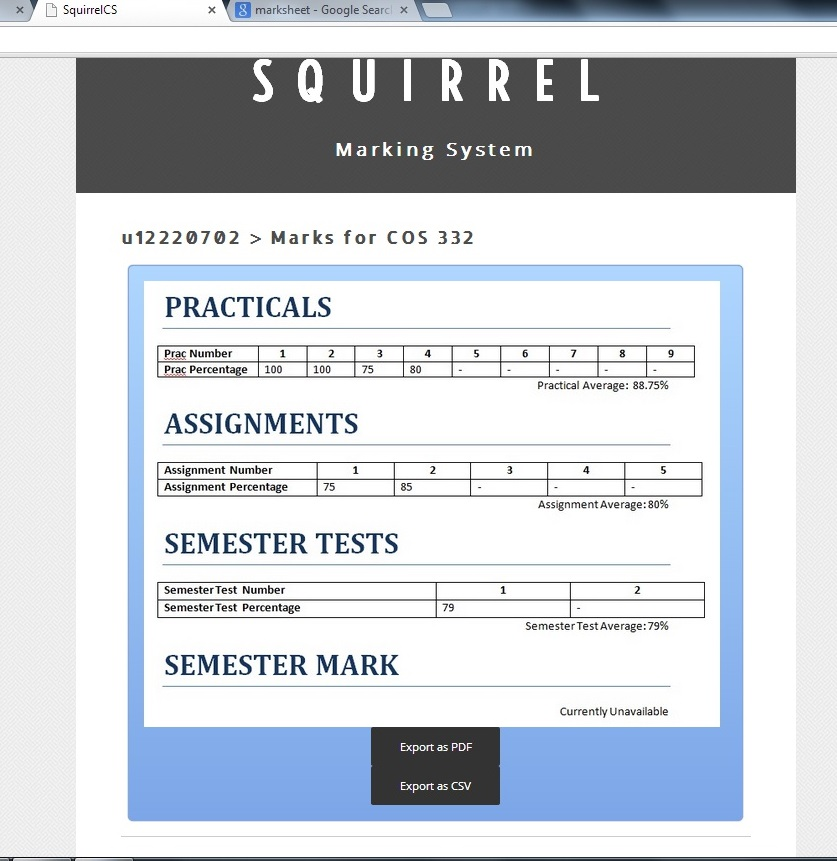
\includegraphics[width=380px]{Images/WEBUIStudent_ViewMarks.jpg}
\begin{center}
Figure 15: And then view all the current marks for that module once the lecturer has released them.
\end{center}
\subsection*{UML Diagrams}
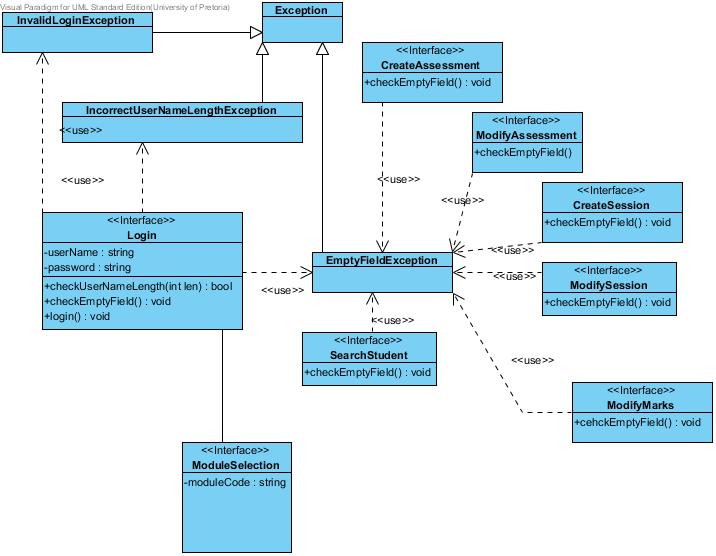
\includegraphics[width=380px]{Images/WEBUML.jpg}
\begin{center}
Figure 16: All possible exceptions for an empty field or student number of invalid length.
\end{center}

\subsection{Android Application}
\subsection*{Detailed System-Process Specifications for Android}
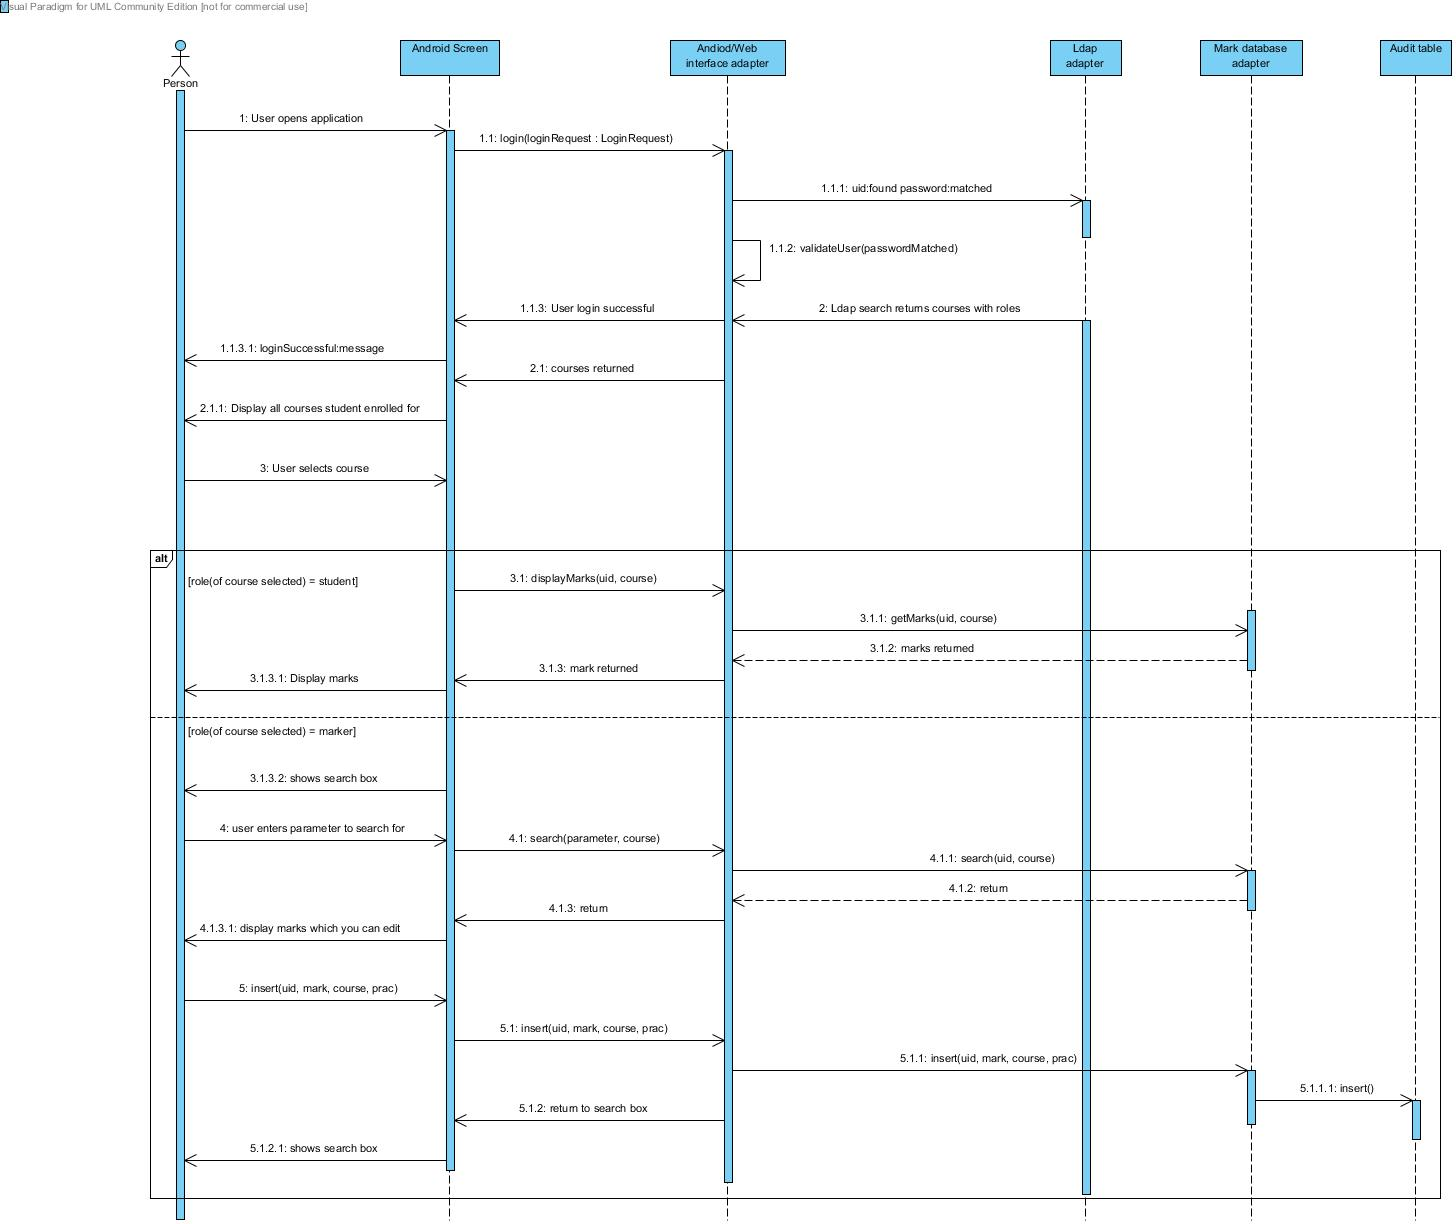
\includegraphics[width=380px]{Images/APPsequence.jpg}
\begin{center}
Figure 17: Android App Sequence Diagram.
\end{center}
This sequence diagram covers the system-process specifications for android application. When the user opens the application the user will be prompted with a login screen. The user will login. The details he entered will be sent to interface(to let the android application and web interface connect an adapter/interface to improve flexibility, if for example ios application wants to be developed will be easier to integrate it with current system).\\
This interface will then communicate with ldap adapter to authenticate the user. Then personal details will be constructed displaying by course this will be provided by ldap since all that information is stored there.\\
For example(Appendices in master specification):\\
LDAP search for memberuid=u29052735 returns:\\

cn: stud COS333\\
cn: stud COS301\\
cn: stud COS326\\
cn: stud COS216\\
cn: stud COS330\\

User can select course that the user is enrolled for or marker or lecturer of. The sequence diagram alt is for when user is a student or when user is a marker. The reason for the course selector is since users can both be markers and students on different courses.  If user is a marker his marks will be fetched by the mark database adapter and then will be sent to the interface and then will be displayed on android application.\\
If user is marker then search box will appear where marker can search students or names. He will only be able to search for students in his assigned practical groups. Then practical’s that are not currently locked that needs to be marked will be available for that student and marker can enter mark. Update must be made in audit-table when any mark is changed.


\subsection*{UI Screen Designs and Work-Flow Specifications}
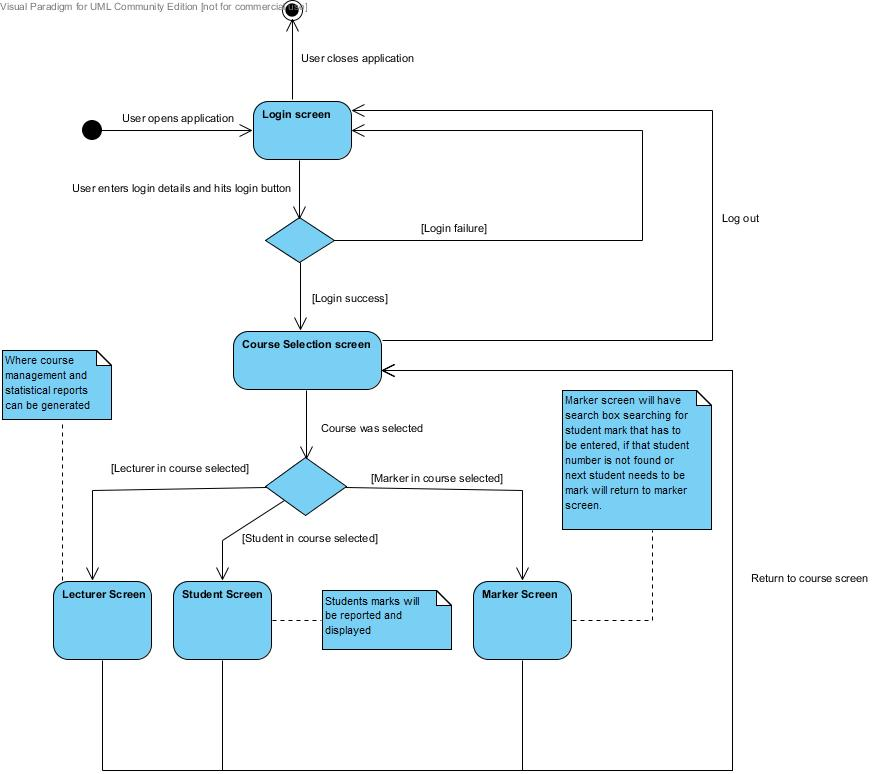
\includegraphics[width=380px]{Images/APPUI1.jpg}
\begin{center}
Figure 18: Android App Activity Diagram.
\end{center}

This is activity diagram of the flow of how the user interface of the android application should work. The rest of the android application layout will not be specified in detail like where the textboxes should be located since we want to keep the user interface flexible for implementation phase and don’t want to tie down and limit the implementation.

\subsection*{Lower Levels of Granularity}
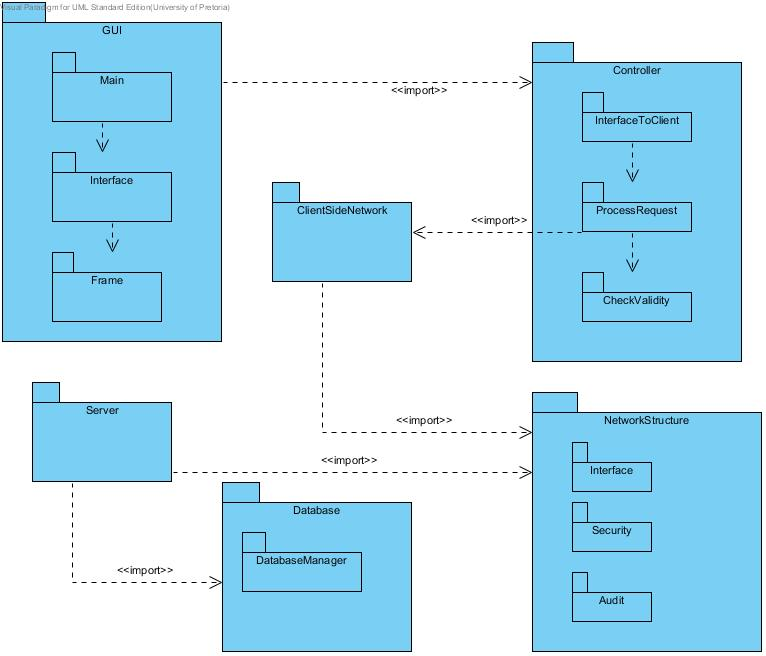
\includegraphics[width=380px]{Images/APPGRANULARITY.jpg}
\begin{center}
Figure 19: Android App Lower Levels of Granularity.
\end{center}

\subsection*{API Specifications}
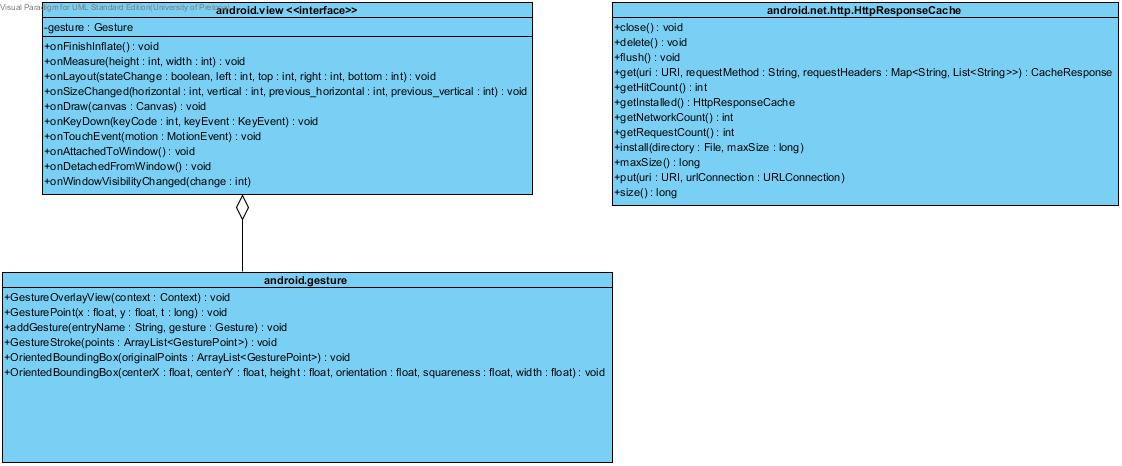
\includegraphics[width=380px]{Images/APPAPI.jpg}
\begin{center}
Figure 20: Android App API.
\end{center}

\subsection*{Class Diagrams}
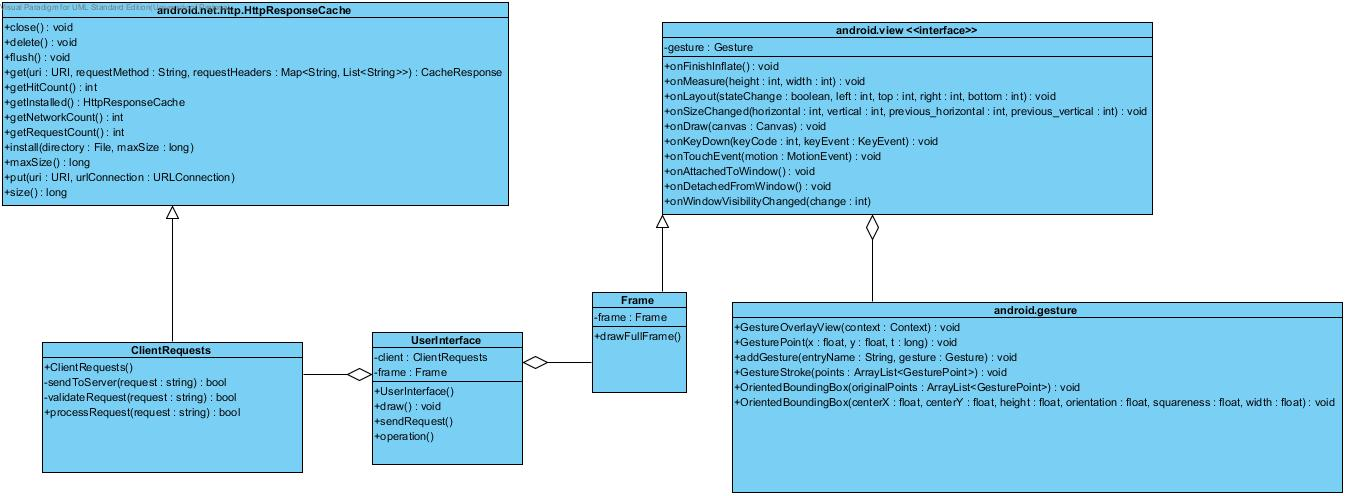
\includegraphics[width=380px]{Images/APPCD.jpg}
\begin{center}
Figure 21: Android App Class Diagrams.
\end{center}

\subsection*{Design of the Database Tables}
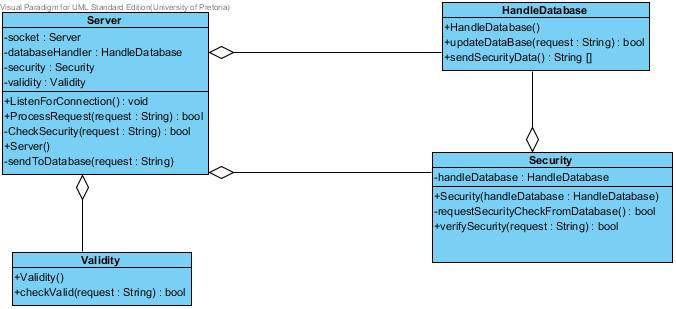
\includegraphics[width=380px]{Images/APPCDS.jpg}
\begin{center}
Figure 22: Android App Class Diagrams for the Server.
\end{center}

\end{document}